%%%%%%%%%%%%%%%%%%%%%%%%%%%%%%%%%%%%%%%%%%%%%%%%%%%%%%%%%%%%%%%%%%%%%%%%%%%%
% AGUJournalTemplate.tex: this template file is for articles formatted with LaTeX
%
% This file includes commands and instructions
% given in the order necessary to produce a final output that will
% satisfy AGU requirements, including customized APA reference formatting.
%
% You may copy this file and give it your
% article name, and enter your text.
%
%
% Step 1: Set the \documentclass
%
%

%% To submit your paper:
\documentclass[draft]{agujournal2019}
\usepackage{url} %this package should fix any errors with URLs in refs.
\usepackage{lineno}
\usepackage[inline]{trackchanges} %for better track changes. finalnew option will compile document with changes incorporated.
\usepackage{soul}
\usepackage{amsmath}
\usepackage{siunitx}
\usepackage{color}
\newcommand{\red}[1]{\textcolor{red}{#1}}
\newcommand{\blue}[1]{\textcolor{blue}{#1}}

\linenumbers
%%%%%%%
% As of 2018 we recommend use of the TrackChanges package to mark revisions.
% The trackchanges package adds five new LaTeX commands:
%
%  \note[editor]{The note}
%  \annote[editor]{Text to annotate}{The note}
%  \add[editor]{Text to add}
%  \remove[editor]{Text to remove}
%  \change[editor]{Text to remove}{Text to add}
%
% complete documentation is here: http://trackchanges.sourceforge.net/
%%%%%%%

\draftfalse

%% Enter journal name below.
%% Choose from this list of Journals:
%
% JGR: Atmospheres
% JGR: Biogeosciences
% JGR: Earth Surface
% JGR: Oceans
% JGR: Planets
% JGR: Solid Earth
% JGR: Space Physics
% Global Biogeochemical Cycles
% Geophysical Research Letters
% Paleoceanography and Paleoclimatology
% Radio Science
% Reviews of Geophysics
% Tectonics
% Space Weather
% Water Resources Research
% Geochemistry, Geophysics, Geosystems
% Journal of Advances in Modeling Earth Systems (JAMES)
% Earth's Future
% Earth and Space Science
% Geohealth
%
% ie, \journalname{Water Resources Research}

\journalname{JGR: Oceans}


\begin{document}

%% ------------------------------------------------------------------------ %%
%  Title
%
% (A title should be specific, informative, and brief. Use
% abbreviations only if they are defined in the abstract. Titles that
% start with general keywords then specific terms are optimized in
% searches)
%
%% ------------------------------------------------------------------------ %%



\title{=enter title here=}

%% ------------------------------------------------------------------------ %%
%
%  AUTHORS AND AFFILIATIONS
%
%% ------------------------------------------------------------------------ %%

% Authors are individuals who have significantly contributed to the
% research and preparation of the article. Group authors are allowed, if
% each author in the group is separately identified in an appendix.)

% List authors by first name or initial followed by last name and
% separated by commas. Use \affil{} to number affiliations, and
% \thanks{} for author notes.
% Additional author notes should be indicated with \thanks{} (for
% example, for current addresses).

% Example: \authors{A. B. Author\affil{1}\thanks{Current address, Antartica}, B. C. Author\affil{2,3}, and D. E.
% Author\affil{3,4}\thanks{Also funded by Monsanto.}}

\authors{=list all authors here=}


% \affiliation{1}{First Affiliation}
% \affiliation{2}{Second Affiliation}
% \affiliation{3}{Third Affiliation}
% \affiliation{4}{Fourth Affiliation}

\affiliation{=number=}{=Affiliation Address=}
%(repeat as many times as is necessary)

%% Corresponding Author:
% Corresponding author mailing address and e-mail address:

% (include name and email addresses of the corresponding author.  More
% than one corresponding author is allowed in this LaTeX file and for
% publication; but only one corresponding author is allowed in our
% editorial system.)

% Example: \correspondingauthor{First and Last Name}{email@address.edu}

\correspondingauthor{=name=}{=email address=}

%% Keypoints, final entry on title page.

%  List up to three key points (at least one is required)
%  Key Points summarize the main points and conclusions of the article
%  Each must be 100 characters or less with no special characters or punctuation and must be complete sentences

% Example:
% \begin{keypoints}
% \item	List up to three key points (at least one is required)
% \item	Key Points summarize the main points and conclusions of the article
% \item	Each must be 100 characters or less with no special characters or punctuation and must be complete sentences
% \end{keypoints}

\begin{keypoints}
\item Recent and potential calving of Pine Island Glacier results in significant changes in basal melting
\item Melt pattern changes dampen the stabilizing effect of calving on shelf mass balance
\item Changes in melt pattern promote runaway collapse of Pine Island ice shelf  
\end{keypoints}

%% ------------------------------------------------------------------------ %%
%
%  ABSTRACT and PLAIN LANGUAGE SUMMARY
%
% A good Abstract will begin with a short description of the problem
% being addressed, briefly describe the new data or analyses, then
% briefly states the main conclusion(s) and how they are supported and
% uncertainties.

% The Plain Language Summary should be written for a broad audience,
% including journalists and the science-interested public, that will not have 
% a background in your field.
%
% A Plain Language Summary is required in GRL, JGR: Planets, JGR: Biogeosciences,
% JGR: Oceans, G-Cubed, Reviews of Geophysics, and JAMES.
% see http://sharingscience.agu.org/creating-plain-language-summary/)
%
%% ------------------------------------------------------------------------ %%
\newcommand{\mpryr}{~m~yr\textsuperscript{-1}}


%% \begin{abstract} starts the second page

\begin{abstract}
[ enter your Abstract here ]
\end{abstract}

\section*{Plain Language Summary}
[ enter your Plain Language Summary here or delete this section]


%% ------------------------------------------------------------------------ %%
%
%  TEXT
%
%% ------------------------------------------------------------------------ %%
\section{Introduction}
%we have seen big changes, and they're mostly driven by increased basal melting
\red{BELOW FOR THE REALISTIC PIG SNAPPING, BUT LEAVING FOR NOW AS PROBABLY ADAPTABLE}
Ice sheets and ice shelves, their floating extensions, in the Amundsen sea sector of Antarctica has undergone significant changes in recent years, characterized by an increasing rate of ice loss [Paolo 2015 Science], grounding line retreat and glacier acceleration. These changes have been particularly prominent for Pine Island Ice Sheet in the eastern Amundsen Sea, which experienced a 70\% increase in ice flux and close to doubling of surface velocity between 1974 and 2013~\cite{Mouginot2014GRL}, while its grounding line retreated some 31~km at its centre between 1992 and 2011~\cite{Rignot2014GRL}. Increased basal melting has been implicated as a key driver of these changes [refs]: ice shelves transfer backstress from contact with ice rumples or embayments to the grounded ice upstream (often called buttressing) effectively restraining the grounding ice; thinning ice shelves offer less buttressing to ice sheets [refs Gudmunsson etc -- see pycnocline paper].

%the story is more complicated that simply increased hot water reaching the shelf (why?).  [see rhs of p120 of Heywood 2016]
The underling cause of changes in basal melting are complicated [what have some studies suggested: overall shoaling of pycnocline, warming of CDW layer etc etc] This picture is complicated further in Pine Island Glacier, owing to the presence of a subglacial ridge located several tens of kilometers upstream of the grounding line. This ridge, in combination with the ice shelf lying over it, acts as a topographic barrier restricting the access of mCDW to an inner cavity between the ridge and the grounding line [fig]. The strength of this barrier is highly dependent on the depth of the pycnocline: if the pycnocline is relatively deep, the mCDW layer does not extend to the level of the top of the ridge and melting is significantly reduced compared to when the pycnocline is relatively shallow  and [the interaction between the gap, the plume and the ridge prevents access] [cite De Rydt 2014]; Dutrieux et al. reported that the total freshwater flux from the fast flowing part of Pine Island Glacier in 2009 (when the pycnocline was at its second highest level on record) was more than double its value in 2012 (pycnocline lowest on record).

%another thing we have seen is significant calving events
Pine Island Glacier has also experience several significant calving events in recent years. Calving events are a typical part of the life cycle of an ice shelf: calving and melt make up the dominant contributions to ice sheet mass losses with balance the accumulation experienced upstream in a glacier in equilibrium. For Pine Island Glacier, these events have, however, led to a significant retreat of the ice shelf front (Figure x). At present, the ice shelf front is [some distance] from the subglacial ridge (notably, closer to the subglacial ridge than in 2012). It has been also been suggested that Pine Island ice shelf has been precondition for disintegration by a damage feedback, whereby ice shelf weakening promotes further damage to the ice shelf, resulting in further speedup shearing and weakening. 

%so we might have the scenario whereby the ice shelf retreats beyond the ridge: in this paper we explore the implications of the previous retreat and potential future retreat on the sub-shelf melting of Pine Island
In addition to the significant recently calving, it is therefore conceivable, therefore, that future calving events will retreat the ice shelf close to and beyond the subglacial ridge. Given the importance of the combination of ice shelf and topographic ridge on controlling the melt rate in Pine Island glacier, it is possible that previous and potential future calving events have a significant effect on melting of Pine Island Glacier. In this paper, we aim to explore the implications of this.
\red{Do you want to talk about marine ice cliff instability? Future calving might have already been 'locked in' by previous calving events owing to the MICI.}

%in this paper, we explore the response of melting to calving in an idealized setup. We aim to isolate the physical processes responsible. Idealized modelling also means that 
In this paper, we aim to 



\begin{figure}
    \centering
    \includegraphics{}
    \caption{Info on realistic PIG}
    \label{fig:figure1}
\end{figure}

\section{Experiment Details}
%broad overview of the experiemnts
We perform a total of nine experiments, each corresponding to a unique pair of parameters that characterize the hydrographic forcing, the strength of the barrier provided by the shelf, which are known to be variable in practice (section 1). Within each experiment, we perform ten simulations in which the ocean circulation is resolved explicitly using the MIT general circulation model (MITgcm): the first `default' (or `uncalved') simulation  corresponds to a configuration that captures the essential features of the Pine Island Cavity in 2009, while in the nine further `calving' simulations, sections of the ice shelf in the default run are removed subsequently, thus simulating the effect of calving (we use the word calving henceforth as a proxy for this description). Other than removing sections within each experiment, the ice shelf geometry does not change within each experiment (but may change between experiments, see section \ref{S:Experiment:Geometry}). Ice shelves therefore enter passively, via the exchange of heat and salt at the ice-ocean interface alone; a passive description of ice shelves (i.e. not including any ice sheet or ice shelf dynamics) is sufficient for this study since we are primarily interested in response of melt rates to ice shelf calving, which occur on timescales much shorter than on which the ice responds dynamically to perturbations in melting. In the following sections we provide further details of the ocean model and experimental setup, including the motivation for various parameter choices.

\begin{figure}
    \centering
    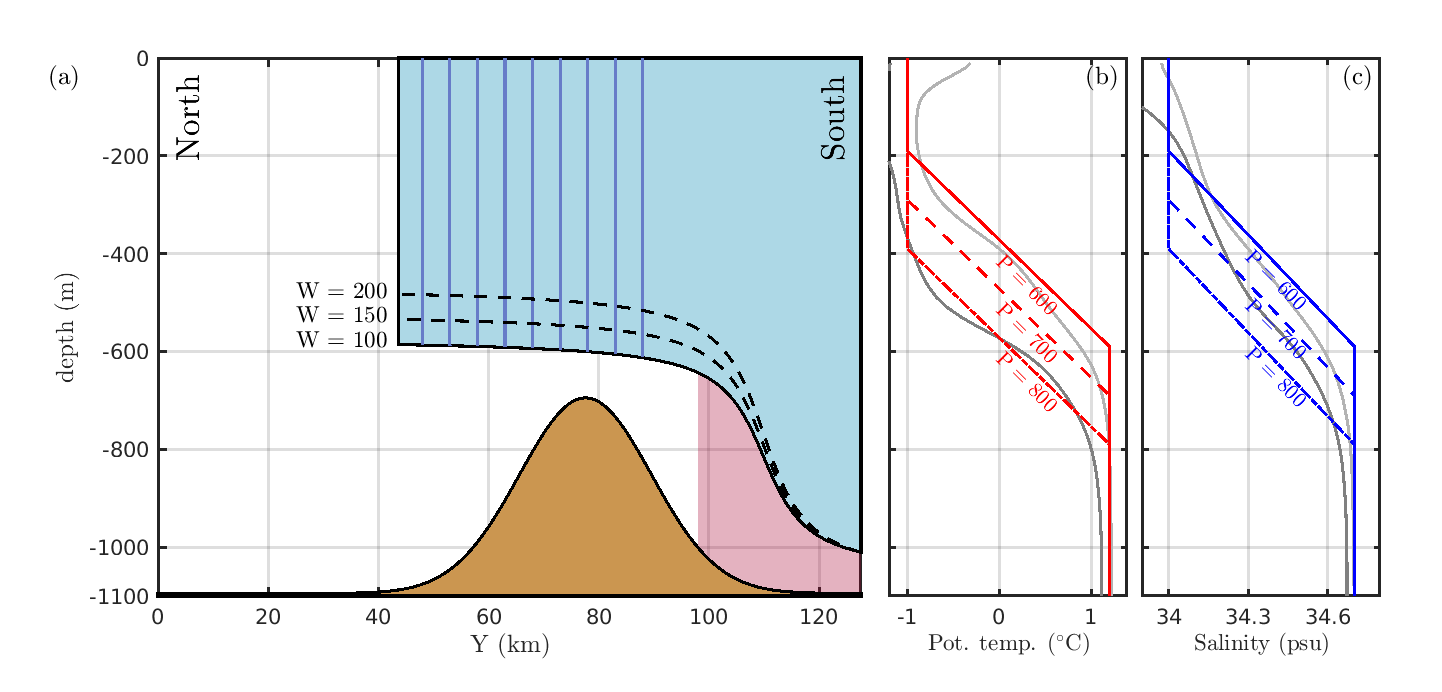
\includegraphics[width = \textwidth]{../make_figures/plots/figure2.eps}
    \caption{(a) Schematic diagram of the experimental setup. The ocean domain consists of the gridded area, which is bordered by a passive ice shelf (shaded blue) and seabed ridge a (shaded brown). Solid and dashed black lines indicate the ice shelf geometry used in the default simulation for the three values of the ridge-gap parameter $H$=100~m, $H$=150~m, and $H$=200~m, as labelled. Solid blue lines indicate the ice front in the calving experiments, which are located 80, 75, 70, 65, 60, 55, 50, 45, and 40~km north of the southern end of the domain. The shaded grey region indicates the `inner cavity' (see main text), which are areas in the ocean domain that are within 30~km of the southern end of the domain. (b) Salinity and temperature profiles used in the experiments (red and blue curves), with $P = 600$ (solid), $P = 700$ (dashed), $P = 800$ (dot-dashed) as indicated by the label. Grey lines correspond to temperature and salinity profiles taken from CTD measurements in Pine Island Bay during the austral summers of 2009 (light grey) and 2012 (dark grey).  \red{Need (a), (b) labels and shade the inner cavity region, change the P800 to dot dashed. Add shaded restoring region.} }
    \label{fig:figure2}
\end{figure}

\subsection{Details of Ocean Model}
The MITgcm is a z-level general circulation model that includes a partial-cell treatment of topography, allowing an accurate description of both the seabed and ice draft. Our model grid consists of 110 layers with a vertical spacing of 10~m, and a horizontal resolution of 400m. We use the MITgcm in hydrostatic mode with a implicit nonlinear free surface scheme, a third-order direct space-time flux limited advection scheme, a non-linear equation of state~\citeA{Mcdougall2003JAtmosOceanTech}, and the Pacanowski-Philander~\cite{Pacanowski1981JPhysOcean} scheme parametrizes vertical mixing. Constant values of 15 and 2.5~m\textsuperscript{2}~s\textsuperscript{-1} are used for the horizontal Laplacian viscosity and horizontal diffusivity. The equations are solved on an $f$-plane with $f = -1.4\times10^{-4}~\text{s}^{-1}$.

Each simulation is ran for a total of 12 months, using a timestep of 30~\si{seconds}, after which time the configuration reaches a steady state. The melt rates reach approximately 95\% of their final values with three months \red{(see Appendix?)}. All results presented here are averaged over months nine to twelve in the simulation. 

The MITgcm includes a static representation of ice shelves~\cite{Losch2008JGeophysResOceans}. Ice shelf melting is implemented using the so-called "three-equation formulation"~\cite{Holland1999JPhysOcean} that describes the exchange of heat and salt across the ice-ocean boundary. The implementation of this scheme in MITgcm has been described in detail elsewhere~\cite[for example]{DeRydt2014JGeophysResOceans,Dansereau2014JGROceans} but we note that thermal exchange across the ice-ocean interface is typically dominated by latent heat (a consequence of the fact that temperatures difference between ice shelves and the adjacent boundary layer is on the order of several degrees Celsius, while the characteristic temperature associated with latent heat removal is -84 degrees Celsius). With latent heat dominate thermal exchange, the three equation formulation gives the melt rate $\dot{m}$ as
\begin{equation}\label{E:MeltRate}
    \dot{m} = \frac{c_p \gamma_T (T - T_b)}{L}.
\end{equation}
Here $c_p = 3947~\si{\joule \kilogram}^{-1}$ is the specific heat capacity of water, $T$ is the temperature of the ambient ocean, $T_b$ is the temperature at the ice shelf base, which must be at the local freezing point, and $\gamma_T$ is a heat exchange co-efficient. The heat exchange coefficient has an approximately linear relationship on $u^*$, the ocean speed adjacent to the ice shelf base~\cite{Holland1999JPhysOcean}; assuming a perfectly linear relationship, equation~\eqref{E:MeltRateUdT} yields
\begin{equation}\label{E:MeltRateUdT}
    \dot{m} \propto u^* (T - T_b).
\end{equation}
We shall return to~\eqref{E:MeltRateUdT} when diagnosing the reasons for changes in the melt rate as the ice shelf calves.

All parameter values used in the three equation formulation here are as in~\citeA{Holland1999JPhysOcean}, with the exception of the drag co-efficient, which is set to $4.5\times10^{-3}$, a value is more appropriate for Pine Island Glacier~\cite{Dutrieux2014Science} (the drag coefficient that enters in the momentum balance, which can be set independently, remains at the default value of $2.5\times 10^{-3}$).

\subsection{Ice Shelf Geometry and Seabed Bathymetry}\label{S:Experiment:Geometry}
Our idealized setup is shown schematically in figure~\ref{fig:figure2}a: it is uniform in the zonal direction, along which the $x$-axis is aligned, and the $y$-axis is aligned along the meridional direction (although PIG is aligned approximately East-West, we assume here that it is aligned East-West, as is standard~\cite{Grosfeld1997JGROceans, DeRydt2014JGeophysResOceans}).

The sea bed has a Gaussian profile,
\begin{equation}\label{E:Experiment:Bed}
    b(x,y) = -1100 + 400 \exp\left[-\frac{\left(y - 50\times 10^3\right)^2}{2\sigma^2}\right],
\end{equation}
where $\sigma = 12$~km is the length scale over which this profile decays towards zero. The profile~\eqref{E:Experiment:Bed} corresponds to a ridge that peaks 50km from the southern end of the domain, which can be considered as the grounding line, at a height of 400m (note that the cavity thickness is prevented from reaching zero at the grounding line as the MITgcm requires at least two grid cells in the vertical to permit horizontal transfer). \blue{Would be nice to add a cross section to figure 2a, of the ice and sea bed along a profile.}

The variability in both Pine Island Ice Shelf draft and the height of the seabed ridge result in a ridge-draft gap that varies between approximately 100m at its narrowest to greater than 300m at it's widest (figure~\ref{fig:figure1}). Since we assumed a constant sea bed geometry, we aim to capture the effect of variability in the ridge-draft gap by considering different values of $H$, the vertical distance between the crest of the seabed ridge and the ice shelf base; $H$ enters only the model only via the ice profile, which, following~\citeA{DeRydt2014JGeophysResOceans}, takes the form
\begin{equation}
    h(y) = \begin{cases}
    \left(\frac{310 + H}{2.64}\right)\tan^{-1}\left(\frac{y}{5882} -3\right) & \text{for}~y < y_f,\\
    0  & \text{for}~y \geq y_f.
    \end{cases}
\end{equation}
Here $y_c$ is the location of the ice front, which is varied in order to simulate calving (see below). We stress that these ice profiles are not obtained from ice dynamics considerations, but do feature a flatter section beyond the ridge and a steeper section inside the ridge that is observed in practice (figure~\ref{fig:figure2}a).

We use three different values of $H$: $H$=100~m, $H$=150~m, and $H$=200m. The smallest value, $H = 100$m, corresponds to the minimum gap between the ice shelf and ridge that is observed in Pine Island (figure~\ref{fig:figure1}), while the largest value, $H$=200m, corresponds to an upper bound, beyond which the melt response to calving is negligible, as we shall see. The third value, $H$=150~m is an intermediate value between $H$ at which the melt rate is highly sensitive and weakly sensitive to calving.

Within each experiment, the vary the front position $y_f$ is systematically reduced by removing sections of ice, to simulate calving. The ten simulations within each experiment use values $y_f$ = 84 (default), 80, 75, 70, 65, 60, 55, 50, 45, and 40~km, which correspond to calved lengths of 0, 4, 9, 14, 19, 24, 29, 34, 39, and 44~km, respectively. There are both pragmatic and physical reasons for this choosing this particular range: the default experiment with $y_f$= 84~km corresponds to the distance of the ice front in PIG in 2009, before significant calving took place in the late 2010s (the calving experiment with $y_f$=xx~km approximately corresponds to the present day ice front position); the lowest value, $y_f$=40~km, is chosen as a compromise between a configuration in which the ice front has calved a significant distance beyond the ridge, which retains a significant area that is shared by each experiment: as we discuss further in \S\ref{S:Baseline}, the area over which melt rates are averaged should be invariant to calving for a rigorous assessment of changes with calving. The computational expense of ocean simulations together with a large number of experiments means that the number of simulations within the range is restricted to ten.

\subsection{Hydrographic Forcing}\label{S:Experiment:Hydrography}

As discussed in \S\ref{S:Introduction}, the presence of a seabed ridge in Pine Island Glacier means that melt rates are particularly sensitive to the ocean state in the far away from the cavity (the hydrographic forcing); we therefore expect that the melting response to calving will also have a sensitive dependence on hydrographic forcing. To assess this sensitivity, we repeat each of the experiments with different values of the ridge-gap parameter $H$ described in the previous section with three different hydrographic forcings, which are imposed on the model by means of a restoring boundary condition at the northern end of the domain (figure~\ref{fig:figure2}): at this boundary, the temperature and salinity are restored to specified vertical profiles over a distance of five horizontal grid cells (total length 2km) with a restoring timescale that varies from 12~h at the boundary to 60~h at the interior of this restoring regions. (The model includes solid walls with a free slip condition at the southern, western, and eastern sides of the domain.)

%what do our profiles look like
The three temperature and salinity profiles to which the ocean is restored are shown schematically in figure~\ref{fig:figure2}b,c. Both the temperature and salinity profiles are piecewise linear, with constant conditions in both a lower layer (temperature $1.2~\si{\celcius}$, salinity $34.7$~psu) and upper layer (temperature $-1~\si{\celcius}$, salinity $34$~psu) separated by a pycnocline of thickness 400~m. The pycnocline begins at a variable depth $P$ (a higher $P$ corresponds to a deeper pycnocline), which parametrizes the whole profile; our three hydrographic forcings use $P = 600$, $700$, and $800$. 

%why do we choose these conditions
These piecewise linear profiles correspond to (simplified versions of) typical conditions for the Pine Island Bay~\cite{Jacobs1996GRL, Dutrieux2014Science, Jenkins2018NatureGeo} (see figure~\ref{fig:figure2}a,b). The upper and lower layers are dominated by Winter Water and Modified Circumpolar Deep Water, respectively. A record of hydrographic conditions in the Amundsen Sea indicates significant variability in the depth of the pycnocline varies considerably on interannual timescales~\cite{Dutrieux2014Science}; the profiles with $P = 600$ and $P = 800$ correspond to the years 2009 and 2012, respectively, which span the range of observed conditions: in 2012, the average depth of the pycnocline was at the lowest on record, while in 2009, the average depth of the pycnocline was at the highest on record. 

%wrap up the experiments:\ 
The nine experiments can be uniquely identified by a $(H,P)$ pair, where $H$ $\in \{100, 150, 200\}$ and $P$ $\in \{600, 700, 800\}$. We consider the extreme scenario with the strongest topographic barrier and warmest hydrographic forcing, $(H,P) = (100,600)$ to be the baseline; in the following section, we describe the results of this baseline experiment, before describing in sections~\ref{S:Results:H} and~\ref{S:Results:P} how this picture changes for different values of $H$ and $P$, respectively.

\red{AB first readable to here}
\section{Result for the Baseline Experiments}\label{S:Baseline}
In this section, we describe the results for the baseline experiment with $H = 100$ (the narrowest ridge gap width) and $P = 600$ (the highest pycnocline), corresponding to the solid lines in figure~\ref{fig:Schematic}. We begin by describing the steady state configuration for the uncalved run, and then describe how and why calving changes the inner cavity melt rate.

\subsection{Default Run}
%describe each of what we see: melt rate, general observations
Ice-ocean properties that characterise the default case with $H = 100$ and $P =600$ are shown in figure~\ref{fig:figure3}. Melt rates (figure~\ref{fig:figure3} are mostly below  20~m~yr\textsuperscript{-1} everywhere, except for a region located within 20~km of the grounding line, where maximum melt rates of approximately 120~m~yr\textsuperscript{-1} are seen. The average melt rate over the whole shelf is approximately 20\mpryr, which is lower than we see in practice (approximately 33$\pm$2\mpryr for 2009, to which the $P=600$ case corresponds), but this is in the direction we expect, given that the $H = 100$ cavity corresponds to the tightest topographic control we see anyway applied to the whole cavity.
\red{introduce here the definition of the inner cavity, say why we need an area invariance (with respect to the spatially variable melt rate map we've seen for the default run), and quote the value of mean inner cavity melt rate here.}



%why does the melt rate look like it does
Melt rates depend on both cavity circulation and thermal driving. Circulation is controlled by coriolis, spin up a coriolis driven cyclonic circulation within the inner cavity, directed southward at the eastern boundary (large x) and predominantly westward south of $y =$ 30km. There circulation is strong south of $y = 30$~km, but high melt rates are confined to within $y = 20$~km: this is because the thermal driving is weak upstream of the $y = 20$km because of the rising buoyant melt water plume from this region presents colder ocean conditions to the ice shelf thus reducing $\Delta T$ and thus melting (figure 3e). 

%we can use the bsf 
We can gain further understanding into the behaviour in this default case by considering the bsf (figure 3c). If the flow is geostrophic, then the flow will align with contours of constant $f/h$, which are aligned with lines of constant $y$ (i.e. east west). The ice front provides a pv barrier, restricting flow from the open ocean into the cavity. We see melt rates of up to 50\mpryr at the ice front where we get some hot water access and high velocities as the flow downwells forced by this barrier. Under the ice shelf, the flow is primarily constrained by geometry: the ridge acts as a potential voriticity barrier causing the flow to be deflected to the left as it goes up the ridge. This PV barrier is sufficiently strong that there is little flow able to penetrate across the ridge, with the exception of a strong boundary current at the eastern end of the domain, where flow divergence and relative vorticity permit flow perpendicular to contours of constant column this thickness which is southward (northward) in the east (west). By the same token, the cyclonic circulation that spins up in the inner cavity is strongly constrained. 

Although the inner and outer cavity are almost disconnected in a barotropic sense (as we shall see, this is not the case for larger $H$, when the PV barrier is not as strong), they are still connected via flow of warm water over the ridge. In this high pycnocline case, the melt water plume blocks most of the hot water from the outside but some is able to spill over and into the inner cavity, predominantly via the eastern boundary as discussed above (figure 3c shows that plume extends to top of ridge everywhere except boundary) (we verified that the heat content in the inner cavity is in steady state and it's presence is not the result of the initial conditions). This water is cooled by mixing with the meltwater plume (inner cavity temperatures maximum of approx 0.8C, compared to 1.3C outside the cavity), but still provides significant heat for melting. This hot water access leads to a strong stratification in the inner cavity, which results in a fast circulation there because flow is approximately geostrophic within the cavity. 

The key points are that: (1) we spin up a cyclonic circulation in the inner cavity that strongly constrained by the strong pv barrier that the ridge-shelf provides, (2) melt water plume blocks most access of hot water, but still have some hot water access that permits strong melting close to the grounding line (3) presence of hot water and melt water results in high stratification and thus enhanced melting. Despite this being the end member with a barrier that's expected to be stronger than reality, we still get hot water access, plume coldest inshore of the ridge, and weak hydrographic front forms on the northern slope of the ridge. 

\begin{figure}
    \centering
    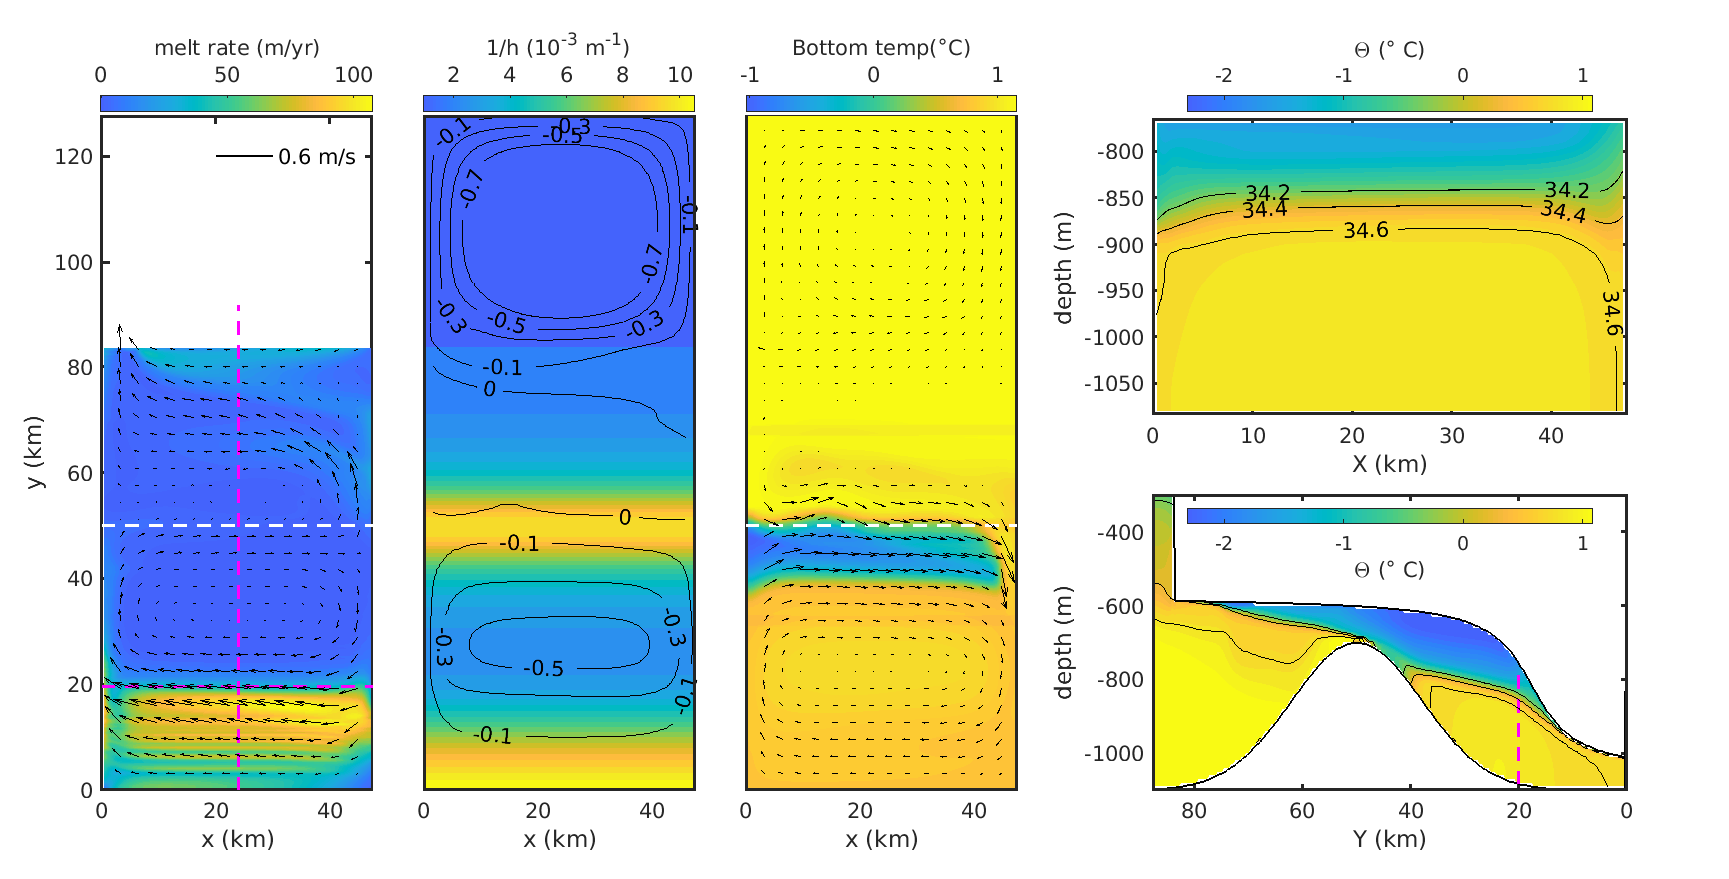
\includegraphics[width = \textwidth]{../make_figures/plots/figure3.eps}
    \caption{Ice-ocean properties that characterize the default (uncalved) run in the baseline experiment ($P = 600$, $H = 100$). (a) Melt rate (colours) and boundary layer velocities (arrows), averaged over the three grid cells adjacent to the ice-ocean interface. White areas correspond to open ocean. Every fifth boundary layer velocity is plotted; the black line indicates an arrow length that would correspond to 0.6~m~s\textsuperscript{-1}. The white dashed line indicates the location of the top of the ridge, while the E-W and N-S aligned dashed magenta lines indicate the location at which the cross sections in (d) and (e) are taken, respectively. (b) Inverse water column thickness (colours) and barotropic stream function (black contours, in units of Sv). (c) Bottom temperature (colours) and bottom current (arrows) averaged over the three grid cells closest to the ocean floor. The scale bar in (a) is also appropriate for (c) \red{check this!}. (d) Zonal cross-section taken along the E-W aligned magenta line in (a), showing potential temperature (colours) and salinity contours at the 34.2, 34.4, and 34.6~psu levels. (e) Meridional cross-section, taken along the N-S aligned magnenta line in (a), with colours and contours as in (d). The magneta dashed line indicates the location of the section correspnding to (d). \red{add a, b, c, d, e labels}}
    \label{fig:figure3}
\end{figure}

%figure 4: plots of (a) melt rate and velocity vectors, (b) geostrophic contours and BSF overlain and (c) bottom current and temperature (i.e. a la Jan 2014 paper)
\subsection{Calving Effect}
As sections of ice are removed from the shelf, the steady state mean melt rate in the inner cavity (henceforth `inner cavity melt rate') changes significantly (figure~\ref{fig:figure4}: it increases rapidly with calving when the ice shelf front is still located beyond the ridge, before suddenly dropping off when the calving event taken the ice front beyond the ridge, reaching an inner cavity melt rate that is approximately independent to further calving. 

In more detail, the mean inner cavity melt rate increases only slightly with calving while the ice shelf front is located a beyond 70~km from the southern end of the domain (calved length less than 14km), but increases significantly at the front retreats further towards the top of the ridge, reaching a maximum of 73\mpryr (70\% larger than the default run) when the ice shelf front is located approximately 5~km north of the ridge crest. As mentioned, a subsequent calving event taking the ice shelf front to directly above the ridge crest (calved length 34km) results in a significant \textit{decrease} of approximately 15$\%$ (from 73\mpryr to 64\mpryr) in the mean inner cavity melt rate. Further calving does not beyond the ridge does not appear to change the mean inner cavity melt rate significantly.

%explain what the Millgate decomposition.
 The melt rate is approximately proportional to the product of the boundary layer velocity and thermal driving (equation~\eqref{E:MeltRateUdT}). We investigate the relative roles of changes in these two quantities in changing the mean inner cavity melt rate by calculating replacing the velocity and thermal driving fields in the calving experiments with the corresponding baseline values, and calculating the resulting mean inner cavity melt rate, relative to the actual melt rate from the simulation. In other words, the effect of changes in boundary layer velocity and thermal driving are assessed by computing
 \begin{equation}\label{E:MillgateDecomp}
U_{\text{effect}} =  \int_{\text{inner cavity}}\frac{u^*(x,y)}{u^*(x,y)_d}, \quad \text{and} \quad \Delta T_{\text{effect}} = \int_{\text{inner cavity}}\frac{T(x,y) - T_f(x,y)}{T_d(x,y) - T_{f,d}(x,y)},
 \end{equation}
  respectively, where subscript d indicates result for the default (uncalved) simulation. The quantities in~\eqref{E:MillgateDecomp} are compared, for a given calving front position, to
 \begin{equation}\label{E:MillgateDecompMelt}
   \mathcal{M} =  \int_{\text{inner cavity}}\frac{u^*(x,y)}{u^*(x,y)_d}.
 \end{equation}
These quantities~\eqref{E:MillgateDecomp} and~\eqref{E:MillgateDecompMelt} are plotted in figure~\ref{fig:figure4}b, where changes in inner cavity melt rate that are driven exclusively by changes in circulation would be indicated by indistinguishable blue and red curves, while changes in the inner cavity melt rate that are driven exclusively by changes in thermal driving at the ice ocean interface would be indicated by indistinguishable blue and green curves. We refer to this comparison as a `velocity-thermal driving decomposition' henceforth.

%what do these plots tell us about what is responsible for the changes?
The velocity-thermal driving composition for the baseline experiments indicates that changes in melting with calving are the result of changes in relative changes in thermal driving and velocity that are of similar magnitude. As the ice front is retreated whilst located outside north of the ridge, both increases in the boundary layer velocity and thermal driving contribute to the increase in melting. When calving beyond the ridge, the thermal driving effect increases, while the velocity effect decreases sharply, indicating a large drop in circulation in the inner cavity. This large drop outweighs the further modest increase in thermal driving effect, leading to an overall reduction in the melt rate when calving beyond the ridge.

%how can we understand what happens.
We gain insight into why the velocity and thermal driving effects behave as described by considering the barotropic stream function and cross sections shown in figure~\ref{fig:figure5}. 
\begin{itemize}
    \item When the front is located beyond the ridge, further calving events do not change the topographic barrier provided by the ridge and so the inner cavity circulation still dominated by a strongly confined cyclonic circulation (first column)
    \item However, snapping in this case reduces the area of the plume (second column), as it is constrained to satisfy the geometry. 
    \item This means that mixing along the boundary wall where warm water enters is reduced, meaning less modified (i.e. warmer) water entering cavity (third column). NB. still little flow over the ridge proper. 
    \item This means that (a) water is warmer in the inner cavity (i.e. more thermal driving) and (b) stronger stratification (third column) which enhances vigour of circulation (i.e. more velocity effect).
    \item When we snap to the ridge crest, two things happen  (1) The pv barrier provided by the ridge crest/ice shelf is relaxed and the circulation connect with one another. The circulation is no longer so strongly confined and thus reduces speed (see column 4, reduce velocity effect). (2): In addition to connected domains meaning more heat access, plume no longer blocks ridge crest (it no longer extends that far!); both of these mean that inner cavity flooded with essentially unmodified cdw. This means that there is more heat available for melting (thermal driving effect increases), but also reduced stratification (reduce velocity effect).
\end{itemize}



%figure 5: (a) plot of mean melt rate as a function of extent and (b) millgate decomposition 
\begin{figure}
    \centering
    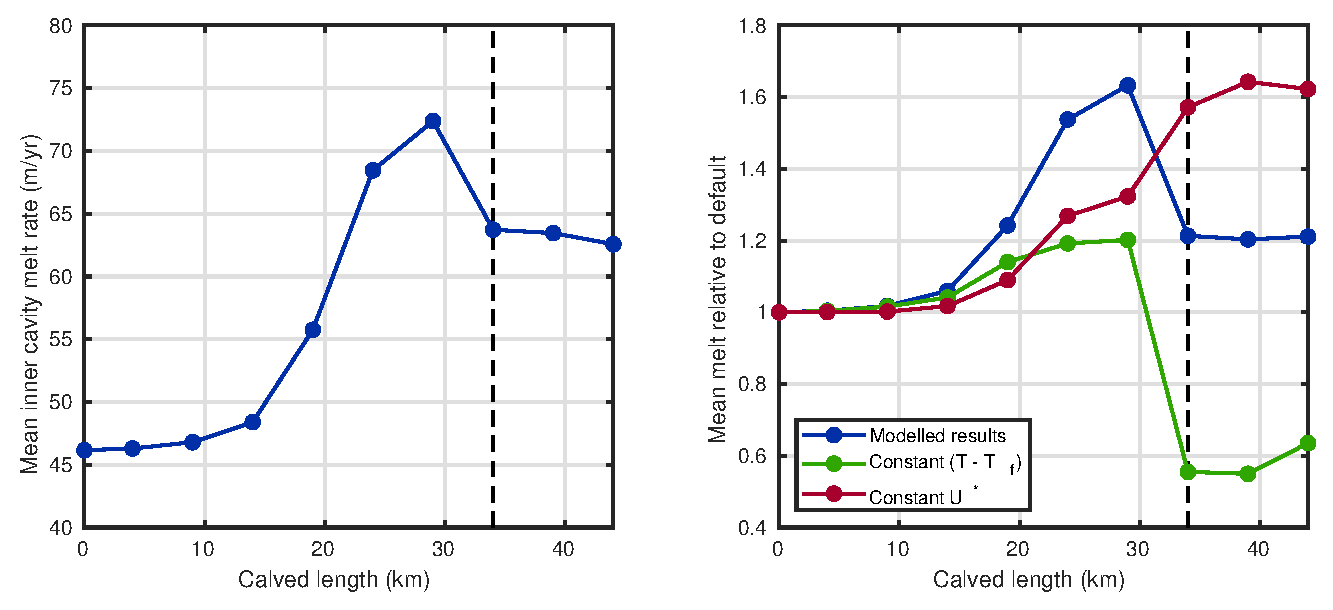
\includegraphics[width = 0.9\textwidth]{../make_figures/plots/figure4.eps}
    \caption{(a) Mean inner cavity melt rate as a function of the calved length of ice. The black dashed line indicates the position of the ice front when it is located directly above the seabed ridge. (b) Velocity-thermal driving decomposition: plot of the decomposition of changes in meean inner cavity melt rate relative to the default (uncalved) experiment (equation~\eqref{E:MillgateDecompMelt}) into changes in boundary layer speed $U_\text{effect}$ (green curve) and thermal driving $\Delta T_{\text{effect}}$ (red curve, see equation~\eqref{E:MillgateDecomp} and main text surrounding).}
    \label{fig:figure4}
\end{figure}

%figure 6: calving with snapping why: (a) row of melt rate (colours) and BSF contours, (b) zonal sections, (c) meridional sections
\begin{figure}
    \centering
    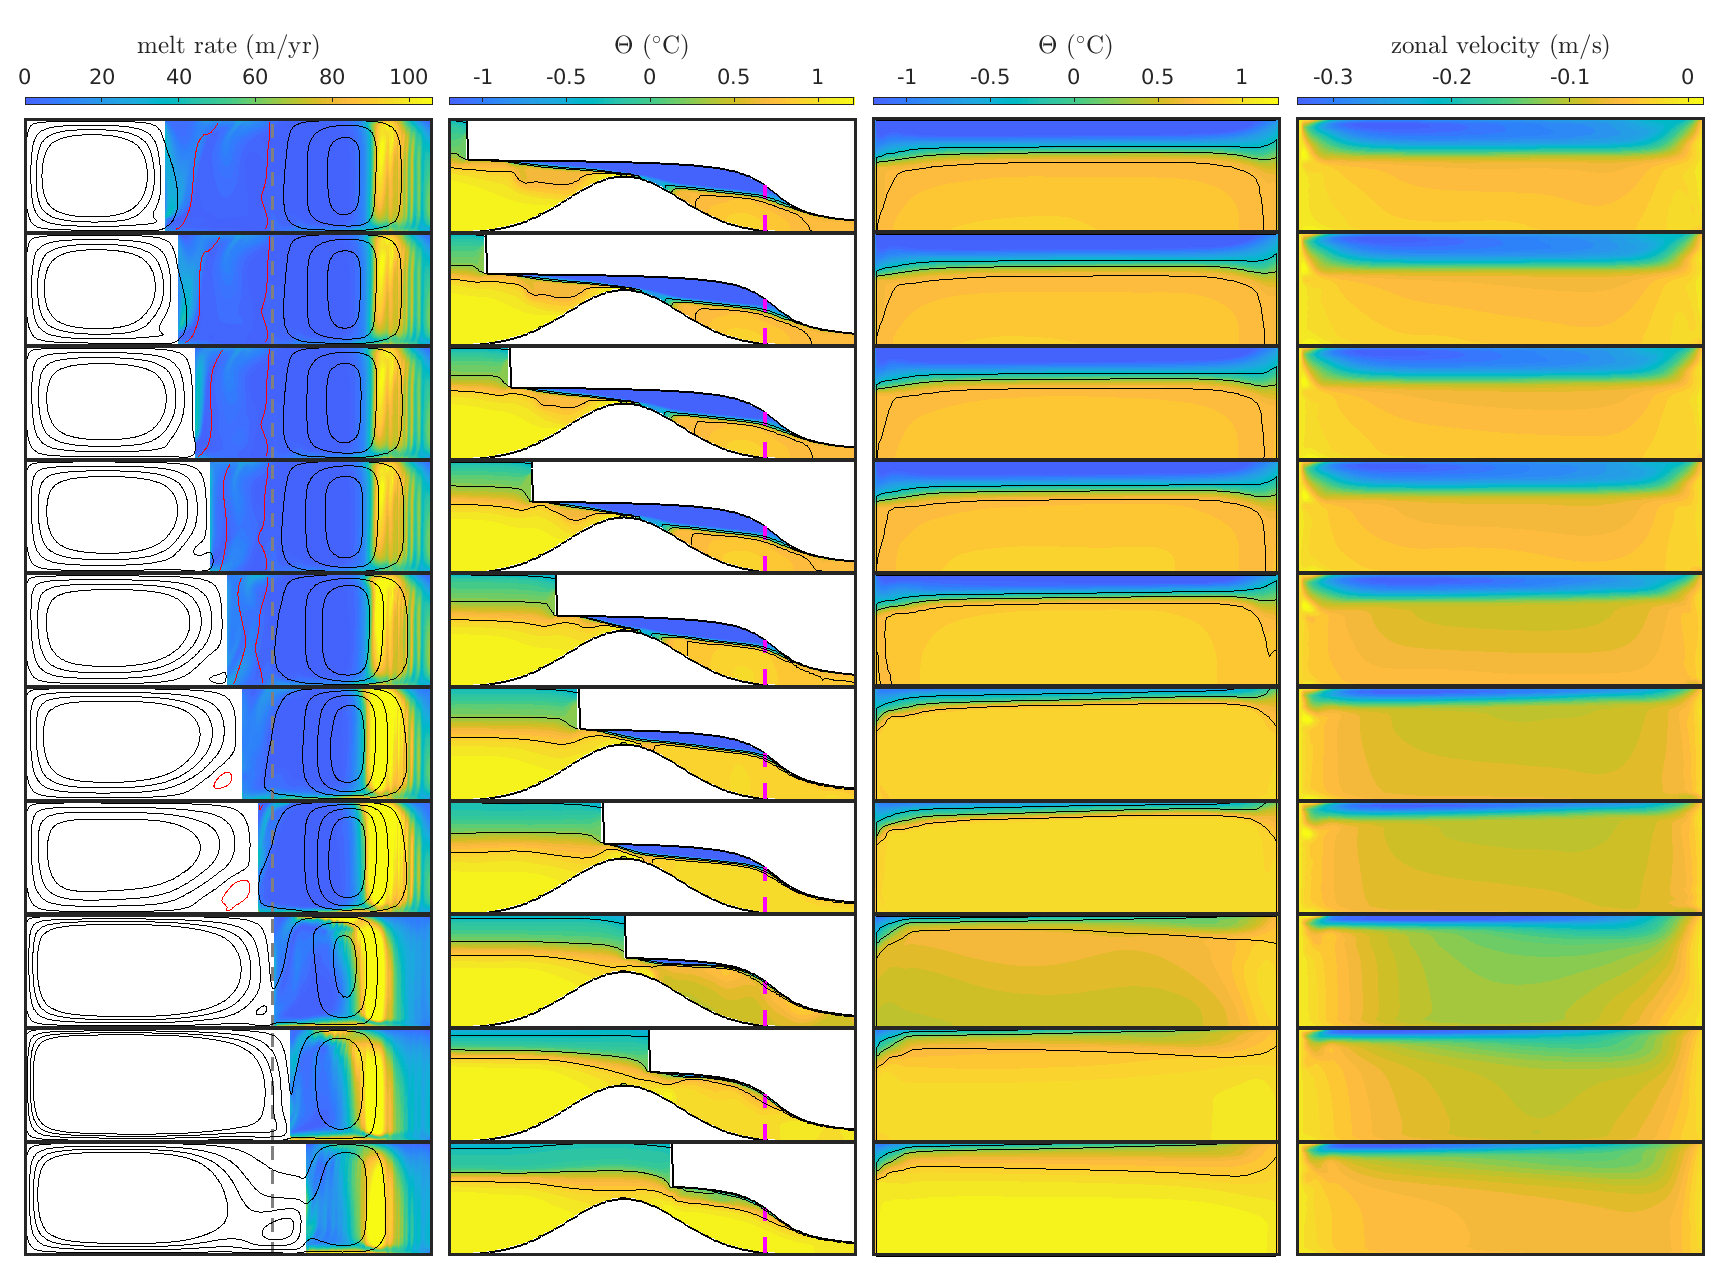
\includegraphics[width = 0.99\textwidth]{../make_figures/plots/figure5.eps}
    \caption{columns showing (a) change of melt rate with snap, (b) meridional cross sectio T and S, (c) zonal cross section T and S, (d) zonal velocity zonal cross section. \red{add a,b,c,d labels for columns and arrow along left with `calving'}}
    \label{fig:figure5}
\end{figure}



\begin{figure}
    \centering
    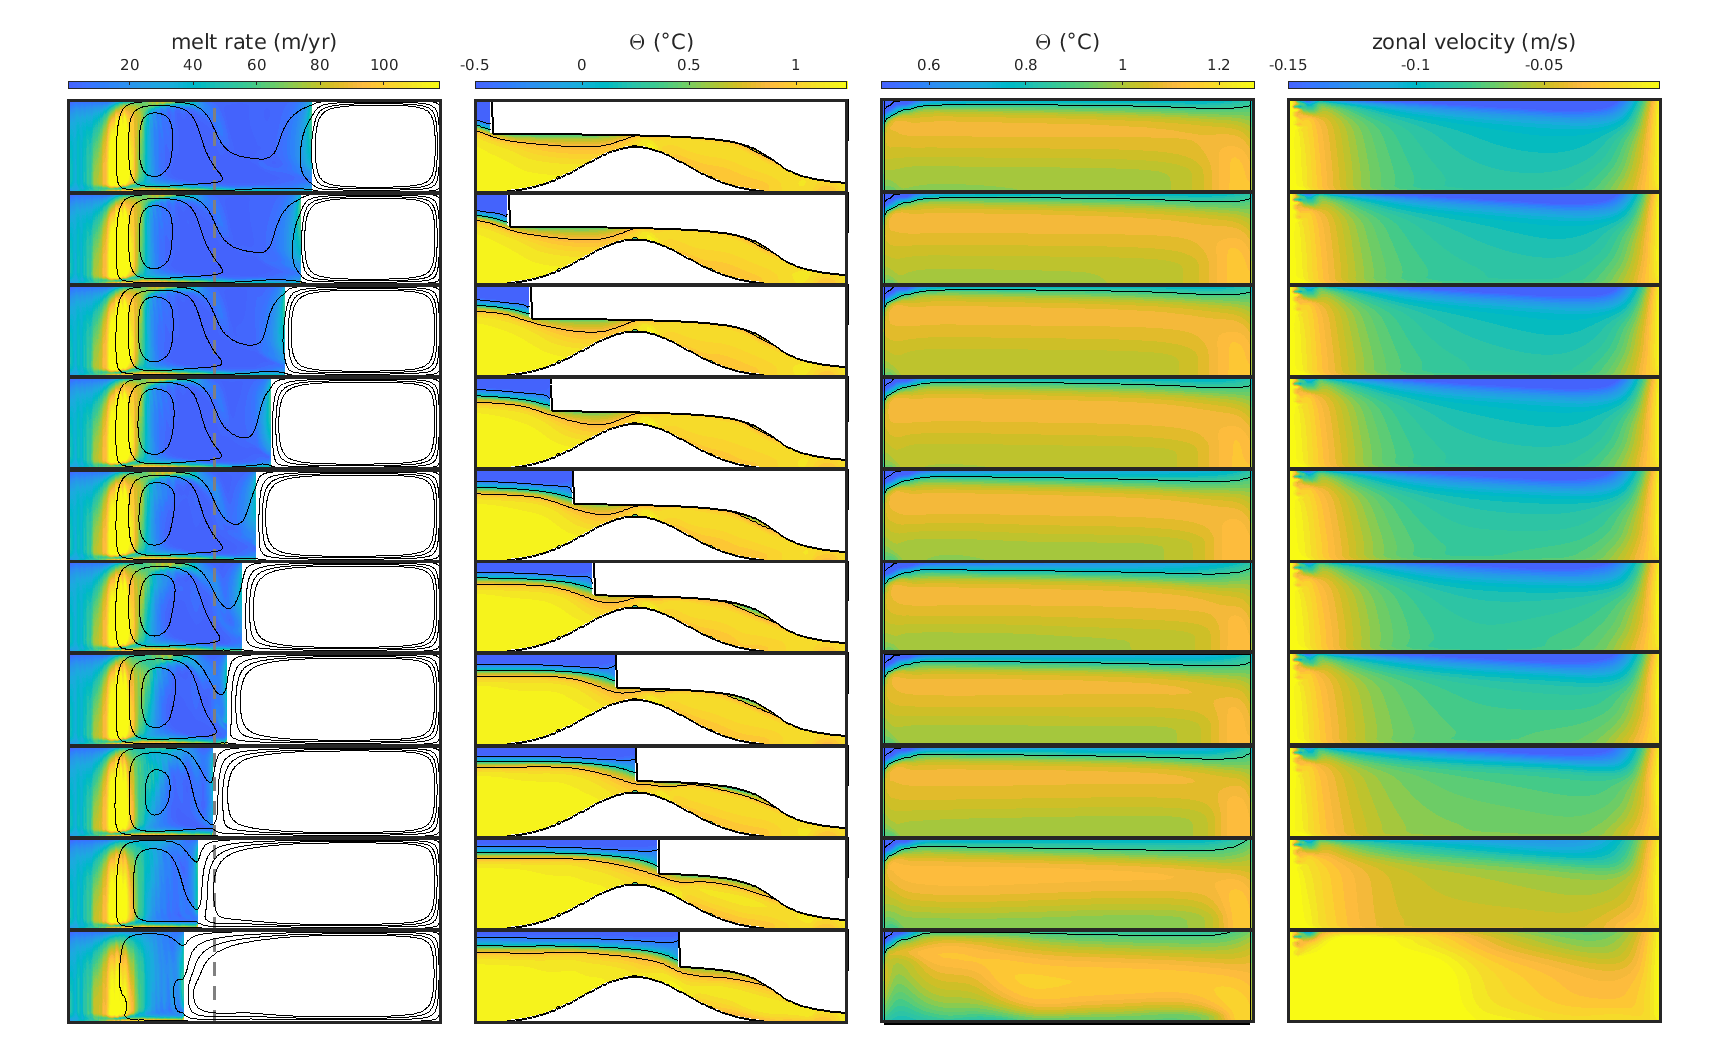
\includegraphics[width = \textwidth]{../make_figures/plots/figure7.eps}
    \caption{Columns as in figure 5 for W = 200 case (note different colour bars in second and third column). \red{needs a,b,c,d labels}}
    \label{fig:figure7}
\end{figure}



\section{Effect of Cavity Geometry on Melt Response to Calving}\label{S:Results:H}
Having understood how and why the inner cavity melt rate changes with calving in the narrow gap $H = 100$ case, we now turn our attention to describing how the picture presented in the previous section changes when the width of the gap, and thus the strength of the topographic barrier provided by the ridge and ice shelf, is increased.

\begin{figure}
    \centering
    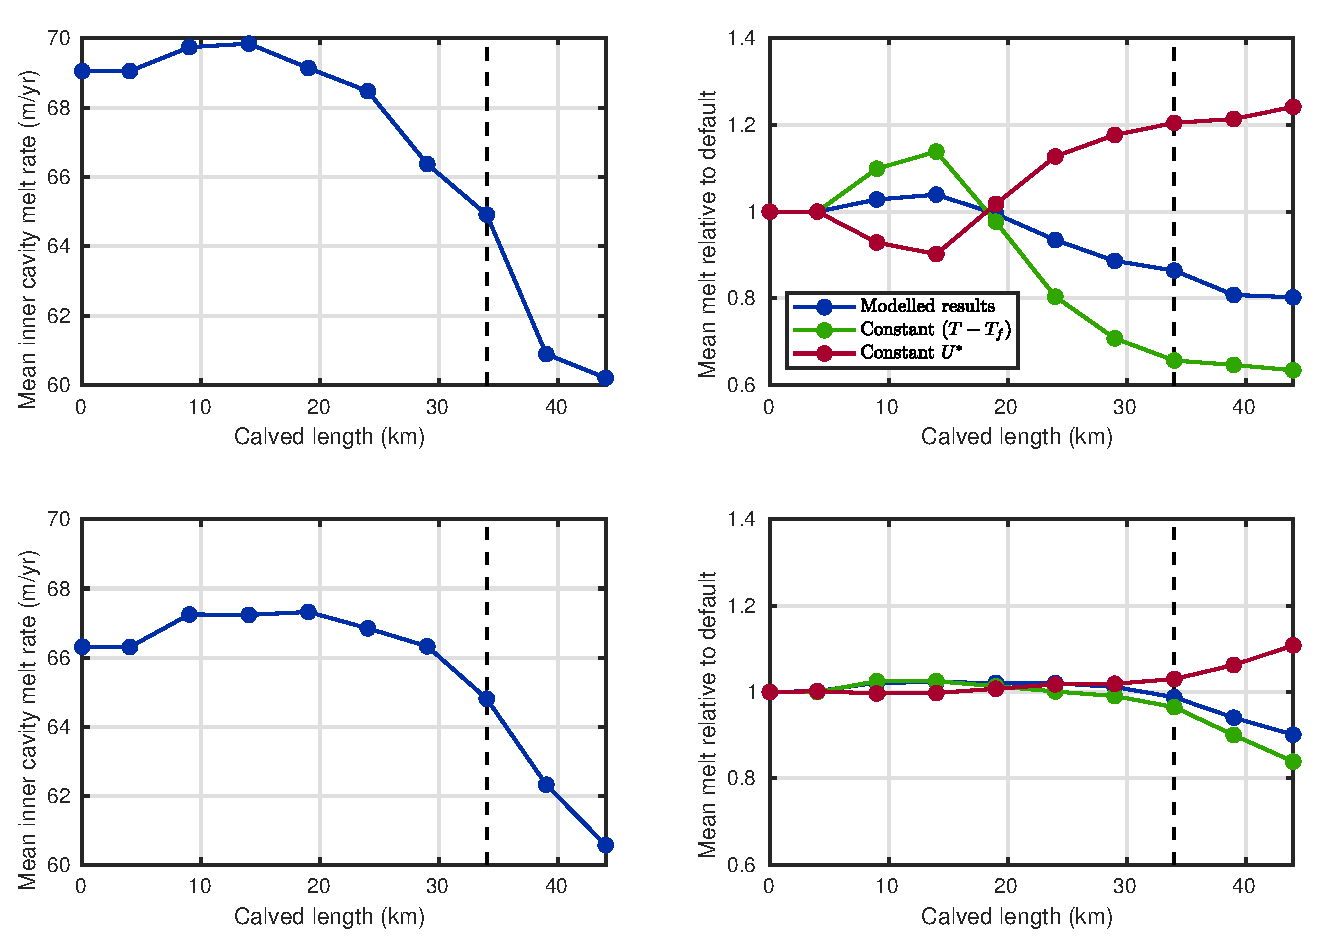
\includegraphics[width = \textwidth]{../make_figures/plots/figure6.eps}
    \caption{Mean melt rate and millgate decomposition for W = 150 and W = 200 \red{NB: two runs missing for W = 150 -- this figure needs updating when we have these done! As do the time limits in the script (change ntout2 from 8 to 12). Could change this to have both mean inner cavity plots on the same axis -- save space and show that effect larger for $W = 200$ than $W = 150$? (also add $W = 100$ results in grey) }}
    \label{fig:figure6}
\end{figure}

%what do we see
Mean melt rates as a function of calved length for the two larger gaps we consider here ($W = 150$~m and $W = 200$~m) are plotted in figure~\ref{fig:figure6}. As in the $W = 100$ case, we see that the melt rate reaches a peak while the ice front is located north of the ridge crest, and further calving events beyond this point reduce the melt rate. From the decomposition, we see in both cases that a reduction in the cavity circulation that outweighs an increase in thermal driving is responsible (and both relative changes are a similar order of magnitude) for the reduction in mean inner cavity melt rate beyond this point.  However, there are several important differences: firstly, the inner cavity melt rate is far less sensitive to calving in both the $W = 150$ and $W = 200$m cases (the difference between largest and smallest inner cavity melt rates is approximately 20\% and 10\%, respectively), and follows the upper end of the maximum range seen in the $W = 100$m case; secondly, the inner cavity melt rate does not show any sort of threshold behaviour when the calving front reaches the top of the ridge.

%why do we see it
To understand the reasons it is useful to compare the cross sections in figure~\ref{fig:figure4} for the $W = 100$ case to the corresponding plot in figure~\ref{fig:figure7} for the $W = 200$ case (a comparison between the $W = 100$m and $W = 150$m case is qualitatively similar to that discussed below for $W = 100$, but the differences are clearer for $W = 200$m.)
\begin{itemize}
    \item Domains are connected even in the default run, and the inner cavity is entirely flushed with warm water. This is different to the `fully' calved $W = 100$m case because the ridge still provides a strong pv barrier constraining the flow to the inner cavity and strongly bounding it, permitting high velocities necessary to allow high mean melt rates.
    \item As we calve, 
\end{itemize}


\section{Effect of Hydrographic Conditions on Melt Response to Calving}\label{S:Results:P}

\section{Discussion}

\section{Summary and Conclusions}



%%% Suggested section heads:
% \section{Introduction}
%
% The main text should start with an introduction. Except for short
% manuscripts (such as comments and replies), the text should be divided
% into sections, each with its own heading.

% Headings should be sentence fragments and do not begin with a
% lowercase letter or number. Examples of good headings are:

% \section{Materials and Methods}
% Here is text on Materials and Methods.
%
% \subsection{A descriptive heading about methods}
% More about Methods.
%
% \section{Data} (Or section title might be a descriptive heading about data)
%
% \section{Results} (Or section title might be a descriptive heading about the
% results)
%
% \section{Conclusions}


%Text here ===>>>


%%

%  Numbered lines in equations:
%  To add line numbers to lines in equations,
%  \begin{linenomath*}
%  \begin{equation}
%  \end{equation}
%  \end{linenomath*}



%% Enter Figures and Tables near as possible to where they are first mentioned:
%
% DO NOT USE \psfrag or \subfigure commands.
%
% Figure captions go below the figure.
% Table titles go above tables;  other caption information
%  should be placed in last line of the table, using
% \multicolumn2l{$^a$ This is a table note.}
%
%----------------
% EXAMPLE FIGURES
%
% \begin{figure}
% \includegraphics{example.png}
% \caption{caption}
% \end{figure}
%
% Giving latex a width will help it to scale the figure properly. A simple trick is to use \textwidth. Try this if large figures run off the side of the page.
% \begin{figure}
% \noindent\includegraphics[width=\textwidth]{anothersample.png}
%\caption{caption}
%\label{pngfiguresample}
%\end{figure}
%
%
% If you get an error about an unknown bounding box, try specifying the width and height of the figure with the natwidth and natheight options. This is common when trying to add a PDF figure without pdflatex.
% \begin{figure}
% \noindent\includegraphics[natwidth=800px,natheight=600px]{samplefigure.pdf}
%\caption{caption}
%\label{pdffiguresample}
%\end{figure}
%
%
% PDFLatex does not seem to be able to process EPS figures. You may want to try the epstopdf package.
%

%
% ---------------
% EXAMPLE TABLE
%
% \begin{table}
% \caption{Time of the Transition Between Phase 1 and Phase 2$^{a}$}
% \centering
% \begin{tabular}{l c}
% \hline
%  Run  & Time (min)  \\
% \hline
%   $l1$  & 260   \\
%   $l2$  & 300   \\
%   $l3$  & 340   \\
%   $h1$  & 270   \\
%   $h2$  & 250   \\
%   $h3$  & 380   \\
%   $r1$  & 370   \\
%   $r2$  & 390   \\
% \hline
% \multicolumn{2}{l}{$^{a}$Footnote text here.}
% \end{tabular}
% \end{table}

%% SIDEWAYS FIGURE and TABLE
% AGU prefers the use of {sidewaystable} over {landscapetable} as it causes fewer problems.
%
% \begin{sidewaysfigure}
% \includegraphics[width=20pc]{figsamp}
% \caption{caption here}
% \label{newfig}
% \end{sidewaysfigure}
%
%  \begin{sidewaystable}
%  \caption{Caption here}
% \label{tab:signif_gap_clos}
%  \begin{tabular}{ccc}
% one&two&three\\
% four&five&six
%  \end{tabular}
%  \end{sidewaystable}

%% If using numbered lines, please surround equations with \begin{linenomath*}...\end{linenomath*}
%\begin{linenomath*}
%\begin{equation}
%y|{f} \sim g(m, \sigma),
%\end{equation}
%\end{linenomath*}

%%% End of body of article

%%%%%%%%%%%%%%%%%%%%%%%%%%%%%%%%
%% Optional Appendix goes here
%
% The \appendix command resets counters and redefines section heads
%
% After typing \appendix
%
%\section{Here Is Appendix Title}
% will show
% A: Here Is Appendix Title
%
%\appendix
%\section{Here is a sample appendix}

%%%%%%%%%%%%%%%%%%%%%%%%%%%%%%%%%%%%%%%%%%%%%%%%%%%%%%%%%%%%%%%%
%
% Optional Glossary, Notation or Acronym section goes here:
%
%%%%%%%%%%%%%%
% Glossary is only allowed in Reviews of Geophysics
%  \begin{glossary}
%  \term{Term}
%   Term Definition here
%  \term{Term}
%   Term Definition here
%  \term{Term}
%   Term Definition here
%  \end{glossary}

%
%%%%%%%%%%%%%%
% Acronyms
%   \begin{acronyms}
%   \acro{Acronym}
%   Definition here
%   \acro{EMOS}
%   Ensemble model output statistics
%   \acro{ECMWF}
%   Centre for Medium-Range Weather Forecasts
%   \end{acronyms}

%
%%%%%%%%%%%%%%
% Notation
%   \begin{notation}
%   \notation{$a+b$} Notation Definition here
%   \notation{$e=mc^2$}
%   Equation in German-born physicist Albert Einstein's theory of special
%  relativity that showed that the increased relativistic mass ($m$) of a
%  body comes from the energy of motion of the body—that is, its kinetic
%  energy ($E$)—divided by the speed of light squared ($c^2$).
%   \end{notation}




%%%%%%%%%%%%%%%%%%%%%%%%%%%%%%%%%%%%%%%%%%%%%%%%%%%%%%%%%%%%%%%%
%
%  ACKNOWLEDGMENTS
%
% The acknowledgments must list:
%
% >>>>	A statement that indicates to the reader where the data
% 	supporting the conclusions can be obtained (for example, in the
% 	references, tables, supporting information, and other databases).
%
% 	All funding sources related to this work from all authors
%
% 	Any real or perceived financial conflicts of interests for any
%	author
%
% 	Other affiliations for any author that may be perceived as
% 	having a conflict of interest with respect to the results of this
% 	paper.
%
%
% It is also the appropriate place to thank colleagues and other contributors.
% AGU does not normally allow dedications.


\acknowledgments
Enter acknowledgments, including your data availability statement, here.


%% ------------------------------------------------------------------------ %%
%% References and Citations

%%%%%%%%%%%%%%%%%%%%%%%%%%%%%%%%%%%%%%%%%%%%%%%
%
% \bibliography{<name of your .bib file>} don't specify the file extension
%
% don't specify bibliographystyle
%%%%%%%%%%%%%%%%%%%%%%%%%%%%%%%%%%%%%%%%%%%%%%%

\bibliography{mybib}



%Reference citation instructions and examples:
%
% Please use ONLY \cite and \citeA for reference citations.
% \cite for parenthetical references
% ...as shown in recent studies (Simpson et al., 2019)
% \citeA for in-text citations
% ...Simpson et al. (2019) have shown...
%
%
%...as shown by \citeA{jskilby}.
%...as shown by \citeA{lewin76}, \citeA{carson86}, \citeA{bartoldy02}, and \citeA{rinaldi03}.
%...has been shown \cite{jskilbye}.
%...has been shown \cite{lewin76,carson86,bartoldy02,rinaldi03}.
%... \cite <i.e.>[]{lewin76,carson86,bartoldy02,rinaldi03}.
%...has been shown by \cite <e.g.,>[and others]{lewin76}.
%
% apacite uses < > for prenotes and [ ] for postnotes
% DO NOT use other cite commands (e.g., \citet, \citep, \citeyear, \nocite, \citealp, etc.).
%



\end{document}



More Information and Advice:

%% ------------------------------------------------------------------------ %%
%
%  SECTION HEADS
%
%% ------------------------------------------------------------------------ %%

% Capitalize the first letter of each word (except for
% prepositions, conjunctions, and articles that are
% three or fewer letters).

% AGU follows standard outline style; therefore, there cannot be a section 1 without
% a section 2, or a section 2.3.1 without a section 2.3.2.
% Please make sure your section numbers are balanced.
% ---------------
% Level 1 head
%
% Use the \section{} command to identify level 1 heads;
% type the appropriate head wording between the curly
% brackets, as shown below.
%
%An example:
%\section{Level 1 Head: Introduction}
%
% ---------------
% Level 2 head
%
% Use the \subsection{} command to identify level 2 heads.
%An example:
%\subsection{Level 2 Head}
%
% ---------------
% Level 3 head
%
% Use the \subsubsection{} command to identify level 3 heads
%An example:
%\subsubsection{Level 3 Head}
%
%---------------
% Level 4 head
%
% Use the \subsubsubsection{} command to identify level 3 heads
% An example:
%\subsubsubsection{Level 4 Head} An example.
%
%% ------------------------------------------------------------------------ %%
%
%  IN-TEXT LISTS
%
%% ------------------------------------------------------------------------ %%
%
% Do not use bulleted lists; enumerated lists are okay.
% \begin{enumerate}
% \item
% \item
% \item
% \end{enumerate}
%
%% ------------------------------------------------------------------------ %%
%
%  EQUATIONS
%
%% ------------------------------------------------------------------------ %%

% Single-line equations are centered.
% Equation arrays will appear left-aligned.

Math coded inside display math mode \[ ...\]
 will not be numbered, e.g.,:
 \[ x^2=y^2 + z^2\]

 Math coded inside \begin{equation} and \end{equation} will
 be automatically numbered, e.g.,:
 \begin{equation}
 x^2=y^2 + z^2
 \end{equation}


% To create multiline equations, use the
% \begin{eqnarray} and \end{eqnarray} environment
% as demonstrated below.
\begin{eqnarray}
  x_{1} & = & (x - x_{0}) \cos \Theta \nonumber \\
        && + (y - y_{0}) \sin \Theta  \nonumber \\
  y_{1} & = & -(x - x_{0}) \sin \Theta \nonumber \\
        && + (y - y_{0}) \cos \Theta.
\end{eqnarray}

%If you don't want an equation number, use the star form:
%\begin{eqnarray*}...\end{eqnarray*}

% Break each line at a sign of operation
% (+, -, etc.) if possible, with the sign of operation
% on the new line.

% Indent second and subsequent lines to align with
% the first character following the equal sign on the
% first line.

% Use an \hspace{} command to insert horizontal space
% into your equation if necessary. Place an appropriate
% unit of measure between the curly braces, e.g.
% \hspace{1in}; you may have to experiment to achieve
% the correct amount of space.


%% ------------------------------------------------------------------------ %%
%
%  EQUATION NUMBERING: COUNTER
%
%% ------------------------------------------------------------------------ %%

% You may change equation numbering by resetting
% the equation counter or by explicitly numbering
% an equation.

% To explicitly number an equation, type \eqnum{}
% (with the desired number between the brackets)
% after the \begin{equation} or \begin{eqnarray}
% command.  The \eqnum{} command will affect only
% the equation it appears with; LaTeX will number
% any equations appearing later in the manuscript
% according to the equation counter.
%

% If you have a multiline equation that needs only
% one equation number, use a \nonumber command in
% front of the double backslashes (\\) as shown in
% the multiline equation above.

% If you are using line numbers, remember to surround
% equations with \begin{linenomath*}...\end{linenomath*}

%  To add line numbers to lines in equations:
%  \begin{linenomath*}
%  \begin{equation}
%  \end{equation}
%  \end{linenomath*}



